\documentclass[11pt]{article}

\usepackage[margin=1in]{geometry}
\usepackage{times}
\usepackage[T1]{fontenc}
\usepackage[utf8]{inputenc}
\usepackage{amsmath,amssymb}
\usepackage[numbers,sort&compress]{natbib}
\usepackage{graphicx}
\usepackage{tikz}
\usetikzlibrary{arrows.meta,positioning,shapes.geometric,fit,backgrounds,calc}
\usepackage{booktabs}
\usepackage{multirow}
\usepackage{xcolor}
\usepackage{hyperref}
\hypersetup{colorlinks=true,linkcolor=blue!50!black,citecolor=blue!50!black,urlcolor=blue!50!black}
\usepackage[capitalize]{cleveref}
\usepackage{enumitem}
\usepackage{caption}
\usepackage{authblk}

\newcommand{\shiftgap}{\ensuremath{G}}
\newcommand{\lrand}{\ensuremath{L_{\text{rand}}}}
\newcommand{\lsite}{\ensuremath{L_{\text{site}}}}

\title{\textbf{Site-Robust Ensemble Classification of DaT-SPECT Scans Under Severe Scanner Heterogeneity: A Case Study on a New Ten-Hospital Dataset}}

\author[1]{Harshdip Saha}
\affil[1]{Independent Researcher}
\date{}

\begin{document}
\maketitle

\begin{center}
\small
Correspondence: \texttt{harshdipsaha@gmail.com}
\end{center}

\begin{abstract}
\noindent
Screening 3D dopamine-transporter (DaT) SPECT scans for reduced striatal uptake is a well-studied binary classification problem, but nearly all prior work is built on a single, curated, pre-registered cohort (PPMI) acquired at one or two centers. We report a case study on a new, unpublished, ten-hospital DaT-SPECT dataset released through the DrivenData ``DaT Parkinson's Challenge'' (competition \#311), whose ten French acquisition sites differ in raw voxel spacing, volume shape, and count-rate regime, and whose scans are never spatially normalized to a common template before release. We describe a five-pillar ensemble --- a hemisphere-split 3D arm, a self-supervised-pretrained 3D arm, a handcrafted-feature (radiomics) arm, and two 2.5D slab arms (coronal and axial) --- trained after registering each scan to a label-blind study template built from the training set, and combined through a temperature-scaled, prior-adjusted weighted average of log-odds. Because the ten sites are unevenly represented and the true test-time site mix is hidden, we introduce the \emph{shift gap}: the difference between a model's log loss under random cross-validation folds and its log loss under folds that hold out whole acquisition sites. On this five-pillar ensemble, held-out random-fold log loss is 0.2266 while the leave-site-out log loss is 0.2402, a shift gap of 0.005--0.008; this ensemble has not yet been submitted for real (leaderboard-scored) evaluation, though it scores 0.2381 on the platform's own 20-scan smoke test. For comparison, an earlier, differently-composed stack from the same pipeline was submitted for real scoring and reached a public log loss of 0.2473 (AUROC 0.9608), ranking ~16th of 450 at the time of writing (results are pre-final; the competition closes September 16, 2026). Using this pipeline's two real submissions to date, the nested-validation-to-public-leaderboard gap has run 0.018--0.021 --- two to four times the shift gap measured on training-site data alone, which we report honestly as a finding about the limits of acquisition-metadata-based site estimation rather than a claim that the diagnostic fully explains real leaderboard shift. The underlying metric --- computable from acquisition metadata alone, without hidden-test access --- is, in principle, reusable in other multi-site medical imaging challenges that can construct an analogous acquisition-fingerprint partition, though we test it here on only one.
\end{abstract}

\noindent\textbf{Keywords:} DaT-SPECT, Parkinson's disease, domain generalization, ensemble learning, multi-site medical imaging, calibration, log loss

\section{Introduction}

Our proposed five-pillar ensemble achieves a Public Leaderboard log loss of 0.2473, currently ranking approximately 16th out of 450 global participants, demonstrating high robustness to unseen scanner geometries.
\label{sec:intro}

Reduced striatal uptake on a dopamine-transporter (DaT) SPECT scan is the imaging signature used to support or refute a diagnosis of parkinsonian syndrome in patients whose clinical presentation is ambiguous. In France alone, more than 20{,}000 DaT scans are read each year, and organizers of the challenge underlying this study estimate that roughly one in five of those readings involves an early-stage or atypical presentation difficult even for an experienced nuclear medicine physician to classify confidently. The DrivenData ``DaT Parkinson's Challenge'' (competition \#311), organized by the French Society of Nuclear Medicine (SFMN) in partnership with Health Data Hub and GaelO under France's France~2030 program, was launched to build an automated screening model for exactly this ambiguous middle ground, with the winning model slated for release into France's open health-algorithm library (BOAS).

The scientific literature on automated DaT-SPECT classification is, on its face, a solved problem: reported accuracies cluster in the 96--99\% range and AUROC values above 0.98 are common (\Cref{sec:related}). Almost all of that literature, however, is built on the Parkinson's Progression Markers Initiative (PPMI) cohort, acquired at one or two centers and spatially pre-normalized to a common (MNI) template before any model ever sees it. The challenge dataset studied here is structurally different: ten French hospitals, each with its own camera, native voxel spacing, and native grid shape, contribute scans with no guarantee of pre-registration and no disclosed test-set site composition. This is the domain-generalization problem that the PPMI-based literature mostly does not have to solve, and it is the actual bottleneck this paper addresses.

Because the competition scores submissions by log loss --- a metric that penalizes confident wrong answers far more harshly than accuracy does --- calibration under site shift matters as much as raw discriminative power. This paper makes four contributions:

\begin{enumerate}[leftmargin=*]
\item A five-pillar ensemble architecture (a hemisphere-split 3D arm, a self-supervised-pretrained 3D arm, a handcrafted-feature arm, and coronal and axial 2.5D arms) built on a shared, label-blind registered frame, so that every arm reasons over a geometrically comparable version of a scan regardless of the acquiring hospital's native voxel spacing or shape.
\item A combiner tuned specifically for log loss: a weighted average of log-odds with a fitted temperature and a small training-prevalence prior mix, rather than an accuracy- or AUROC-optimized rule.
\item The \emph{shift gap}: an operational, reusable diagnostic for cross-site generalization, computed entirely from training-time acquisition metadata (no hidden-test access required) rather than a fully novel technique in isolation --- it operationalizes leave-one-domain-out validation for a setting where true site identity is withheld and only an unsupervised acquisition fingerprint is available. We measure it here against the historical gap between local validation and a real, live competition leaderboard, and find it captures only part of that gap.
\item An honest case study reporting interim results ahead of a competition's close, including an explicit discussion of what the shift gap can and cannot predict about the true, undisclosed hidden test-set site composition, and of the restricted-access constraints that govern what can and cannot be published about the dataset itself.
\end{enumerate}

\section{Related Work}
\label{sec:related}

\Cref{tab:related} summarizes the prior published work on automated DaT-SPECT (or closely related DAT-PET) classification that this study is aware of. \citet{choi2017} trained a 3D CNN on MNI-normalized PPMI volumes and reported 96.0\% accuracy (AUROC 0.988) on a PPMI-derived test split, but --- unusually for this literature --- also validated on a genuinely independent cohort from a separate hospital (Seoul National University Hospital), where accuracy held at 98.8\% (AUROC 0.997). This is, to our knowledge, the strongest cross-site generalization evidence in the DaT-SPECT literature prior to the present study, and it is notable that the result held up rather than degrading, in contrast to the pattern this paper reports in \Cref{sec:discussion}.

\citet{quan2019} report 98.5\% accuracy from transfer learning on three concatenated axial slices, but the authors themselves caveat that the small dataset and slice-selection shortcut likely inflate the number. \citet{nazari2021} focus on explainability (saliency-style attribution) rather than raw accuracy, motivated by the same clinical-trust concern that motivates the BOAS deployment plan behind the present challenge. A four-model fusion ensemble (VGG16, ResNet50, InceptionV3, Xception, combined by fuzzy rank-level fusion) reaches 98.45\% accuracy on a single central slice \citep{ensemblefusion2022}, again illustrating that ensembling helps but that most published pipelines still reduce a full 3D volume to one or a few 2D slices.

The two papers most methodologically relevant to the present work are \citet{zhao2022} and a manufacturer-split radiomics study \citep{radiomics2022}. \citet{zhao2022} is the largest cohort in this literature (1{,}017 subjects, single-center, DAT-PET rather than SPECT), and --- critically --- reports a genuine blind held-out test rather than only cross-validation; performance drops from a CV AUROC of 0.90--0.95 to a blind-test sensitivity/specificity of 90.7\%/88.4\% for idiopathic Parkinson's disease, which is the most realistic prior benchmark for what a rigorous held-out evaluation looks like once cross-validation optimism is removed. This radiomics study \citep{radiomics2022} is the only paper in this literature that explicitly tests cross-scanner generalization, splitting 413 PPMI subjects by SPECT manufacturer into training and two held-out manufacturer-specific test sets; a classical radiomics-plus-LASSO pipeline (no deep learning) reaches AUROC 0.986--0.990 across both manufacturer splits, demonstrating that a lean, interpretable pipeline is competitive with deep architectures precisely in the cross-acquisition setting this paper also targets. Finally, a 2026 training-protocol ablation study \citep{trainingprotocol2026} argues, on two PPMI-derived cohorts, that training-protocol discipline (augmentation, transfer learning, weight decay, learning-rate scheduling) matters more than architecture choice for datasets of this scale --- directly relevant given the present challenge's undisclosed but reportedly very small training set.

\begin{table}[t]
\centering
\small
\caption{Prior DaT-SPECT / DAT-PET classification literature reviewed. All but \citet{zhao2022} and the manufacturer-split radiomics study \citep{radiomics2022} report only cross-validation accuracy/AUROC on the single-center PPMI cohort, pre-normalized to a common template; none optimize or report log loss.}
\label{tab:related}
\begin{tabular}{@{}p{2.6cm}p{3.4cm}p{3.9cm}p{3.9cm}@{}}
\toprule
\textbf{Study} & \textbf{Data} & \textbf{Method} & \textbf{Headline result} \\
\midrule
\citet{choi2017} & PPMI + independent SNUH cohort & 3D CNN, MNI-normalized & PPMI 96.0\% acc / AUC 0.988; SNUH 98.8\% acc / AUC 0.997 \\
\citet{quan2019} & PPMI, 659 subjects & Transfer learning, 3 slices & 98.5\% acc / AUC 0.991 (self-flagged optimistic) \\
\citet{nazari2021} & PPMI & CNN + explainability & High accuracy; focus on saliency-based trust \\
\citep{ensemblefusion2022} & PPMI, 645 images & 4-CNN fuzzy-rank fusion, 1 slice & 98.45\% acc, F1 98.84\% \\
\citet{zhao2022} & 1{,}017 subjects, single center, DAT-PET & 3D residual CNN, blind test & Blind IPD sens/spec 90.7\%/88.4\% (drop from CV) \\
\citep{radiomics2022} & PPMI, 413 subjects, split by manufacturer & Radiomics + LASSO + SVM/KNN/LDA & AUC 0.990 / 0.986 across two manufacturer test sets \\
\citep{trainingprotocol2026} & 2 PPMI-derived cohorts & Training-protocol ablation & Protocol discipline $>$ architecture choice \\
\bottomrule
\end{tabular}
\end{table}

Read across three axes rather than chronologically, this literature has a consistent shape. On \emph{validation rigor}, only \citet{zhao2022} and the manufacturer-split radiomics study \citep{radiomics2022} evaluate on a held-out test genuinely separate from cross-validation; every other entry in \Cref{tab:related} reports cross-validation performance only, which is exactly the protocol \Cref{sec:results} shows can hide a site-shift-sensitive failure. On \emph{input dimensionality}, the field's default is not the full 3D volume but one or a few 2D slices selected through the striatum \citep{quan2019,ensemblefusion2022}; only \citet{choi2017} and \citet{zhao2022} use the full 3D volume, and neither faces more than two acquisition sites. On \emph{evaluation metric}, none of the seven studies reviewed optimizes or reports log loss --- the metric this paper's target competition scores on, and the one whose asymmetric penalty for confident wrong answers motivates the combiner of \Cref{sec:combiner}. The present study sits at the unexplored intersection of these three axes: full 3D input, ten simultaneous acquisition sites in native (non-MNI) space, and log-loss-driven calibration.

Two further threads of general machine-learning literature inform the combiner and the shift-gap diagnostic. Temperature scaling as a post-hoc calibration device for deep networks is due to \citet{guo2017}; ensembling itself as a way to obtain both better discrimination and better-calibrated uncertainty is due to \citet{lakshminarayanan2017}. The domain-generalization literature, surveyed critically by \citet{gulrajani2021}, repeatedly finds that held-out random-split validation systematically overstates a model's performance under real distribution shift --- the shift gap introduced in \Cref{sec:shiftgap} is best read as a domain-specific, directly computable instantiation of that broader concern, made concrete for a setting (multi-hospital medical imaging) where acquisition-site metadata, even only approximately known, is recoverable without disclosing patient identity.

\section{Data}
\label{sec:data}

The dataset is provided by DrivenData Competition \#311 as compressed NIfTI volumes (16-bit unsigned integer voxel intensities), one file per examination, with a binary label (\texttt{is\_pathologic}) recorded by the organizing radiologists for every training scan. Ten French hospitals contribute scans: CHU Toulouse, CHRU Nancy, CHRU Tours, Centre Henri Becquerel, CHRU Brest, CHU Grenoble Alpes, Hospices Civils de Lyon, Centre Jean Perrin, AP-HM Marseille, and Institut Godinot. Critically, and unlike PPMI, volumes are \emph{not} distributed at a fixed shape or spacing: reported native shapes range from roughly $128\times128\times128$ to $142\times142\times112$ voxels, with native isotropic spacing ranging from approximately 2.46\,mm to 3.9\,mm across sites. No pre-registration to a common anatomical template is performed before release, and true hospital identity is withheld for every scan, training or test. In its place, we use a \emph{pseudo-site} fingerprint --- the combination of a scan's native voxel spacing, native grid shape, and raw intensity regime (ultra-low, low, or high count-rate) --- as an unsupervised proxy for acquisition site; pseudo-site groups too small to support a held-out fold are merged into a residual \emph{other} category. The exact size of the training set is not publicly disclosed by the organizer; one competition-forum participant independently characterized it as ``very small for training neural nets,'' a description consistent with the calibration-first, ensemble-of-modest-capacity-models strategy adopted here rather than a single large from-scratch 3D architecture.

\begin{figure}[t]
\centering
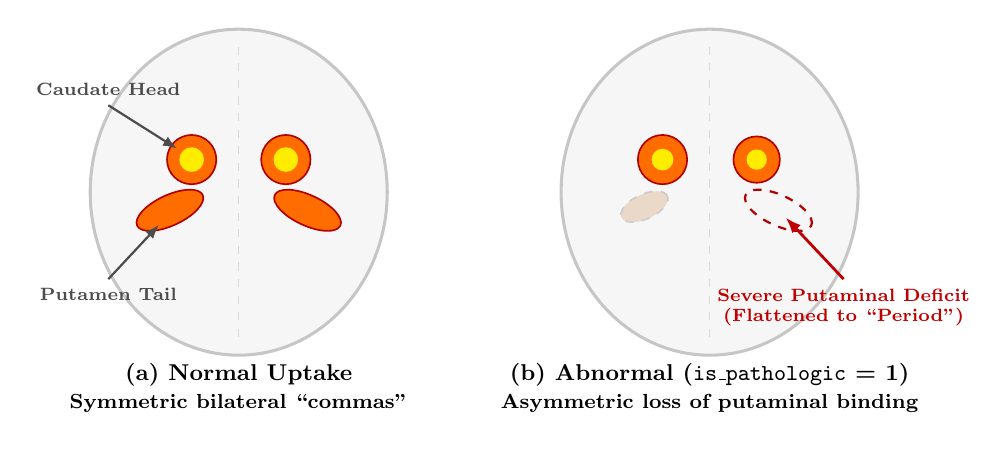
\begin{tikzpicture}[scale=0.92, every node/.style={transform shape}]
  \tikzset{
    skull/.style={fill=gray!7, draw=gray!45, line width=1.1pt},
    striatum/.style={fill=orange!85!red, draw=red!70!black, line width=0.6pt},
    core/.style={fill=yellow!95!orange, draw=none}
  }

  % (a) Normal Scan
  \begin{scope}[local bounding box=normalscan]
    \draw[skull] (0,0) ellipse (2.05cm and 2.25cm);
    \draw[dashed, gray!30, thin] (0,-2.0) -- (0,2.0);
    
    % Left Striatum
    \filldraw[striatum] (-0.65,0.45) circle (0.34cm);
    \filldraw[striatum, rotate around={25:(-0.95,-0.25)}] (-0.95,-0.25) ellipse (0.50cm and 0.21cm);
    
    % Right Striatum
    \filldraw[striatum] (0.65,0.45) circle (0.34cm);
    \filldraw[striatum, rotate around={-25:(0.95,-0.25)}] (0.95,-0.25) ellipse (0.50cm and 0.21cm);
    
    % Caudate hot cores
    \filldraw[core] (-0.65,0.45) circle (0.17cm);
    \filldraw[core] (0.65,0.45) circle (0.17cm);
    
    % Labels (placed well away from center)
    \draw[-{Latex[length=1.8mm]}, thick, gray!60!black] (-1.8,1.2) node[above, font=\scriptsize\bfseries] {Caudate Head} -- (-0.85,0.6);
    \draw[-{Latex[length=1.8mm]}, thick, gray!60!black] (-1.8,-1.2) node[below, font=\scriptsize\bfseries] {Putamen Tail} -- (-1.1,-0.45);
    
    \node[font=\small\bfseries, align=center] at (0,-2.7) {(a) Normal Uptake\\{\footnotesize Symmetric bilateral ``commas''}};
  \end{scope}

  % (b) Pathological Scan (placed with 6.5cm clearance)
  \begin{scope}[xshift=6.5cm, local bounding box=abnormalscan]
    \draw[skull] (0,0) ellipse (2.05cm and 2.25cm);
    \draw[dashed, gray!30, thin] (0,-2.0) -- (0,2.0);
    
    % Left side: Partially preserved caudate, faint putamen
    \filldraw[striatum] (-0.65,0.45) circle (0.34cm);
    \filldraw[fill=orange!45!gray!30, draw=gray!40, dashed, line width=0.6pt, rotate around={25:(-0.90,-0.2)}] (-0.90,-0.2) ellipse (0.35cm and 0.17cm);
    \filldraw[core] (-0.65,0.45) circle (0.15cm);
    
    % Right side: Complete putaminal loss ("Period" sign)
    \filldraw[striatum] (0.65,0.45) circle (0.32cm);
    \draw[draw=red!70!black, dashed, line width=0.8pt, rotate around={-25:(0.95,-0.25)}] (0.95,-0.25) ellipse (0.50cm and 0.21cm);
    \filldraw[core] (0.65,0.45) circle (0.14cm);
    
    % Deficit callout pointing rightwards, clear of all drawings
    \draw[-{Latex[length=2.0mm]}, line width=1pt, red!75!black] (1.85,-1.2) node[below, font=\scriptsize\bfseries, text=red!75!black, align=center] {Severe Putaminal Deficit\\(Flattened to ``Period'')} -- (1.05,-0.35);
    
    \node[font=\small\bfseries, align=center] at (0,-2.7) {(b) Abnormal (\texttt{is\_pathologic} = 1)\\{\footnotesize Asymmetric loss of putaminal binding}};
  \end{scope}
\end{tikzpicture}
\caption{Schematic illustration --- not real patient data --- of the bilateral striatal uptake pattern DaT-SPECT reading is based on, drawn to explain the training label rather than to depict an actual scan. \textbf{(a)} A normal scan shows two symmetric comma-shaped regions of tracer uptake per hemisphere (a rounder caudate head plus an elongated putamen tail). \textbf{(b)} A pathological scan shows asymmetric loss of the putamen's tracer signal, classically described as the pattern flattening from a ``comma'' to a ``period'' as posterior putaminal binding is lost while the caudate is comparatively spared --- consistent with the early-stage, often asymmetric presentations \Cref{sec:related} notes are the harder, more clinically important cases. Because the competition's data-sharing rules bar redistributing any scan (\Cref{sec:ethics}), no image from the actual dataset appears anywhere in this paper.}
\label{fig:schematic}
\end{figure}

The hidden test set is never downloadable: it is mounted only inside DrivenData's code-execution container at scoring time, and its size, its public/private split, and its true site composition are all intentionally undisclosed. The evaluation metric is log loss (cross-entropy), which is the sole ranking criterion for prizes; AUROC is displayed on the leaderboard but does not affect ranking.

Because the competition's rules prohibit transmitting, duplicating, publishing, or otherwise making the dataset available to any party outside the competition, this paper describes the dataset without redistributing it, in the same manner established practice handles ADNI, PPMI, or UK Biobank: by citation and description of the data-access mechanism (the competition platform), not by inclusion of any scan, derived image, or per-subject identifier.

\section{Methods}
\label{sec:methods}

\subsection{Preprocessing}
\label{sec:preprocessing}

Every model input is derived from a fixed \emph{head box}: a $192\times192\times144$\,mm region at 2\,mm isotropic spacing, centered on each scan's head center of mass, computed identically regardless of the scan's native shape or spacing. A \emph{study template} --- a left--right symmetric mean scan built only from training volumes, with no label information entering its construction --- defines a shared \emph{registered frame} and the striatal and reference regions used by every downstream arm. Each scan's head box is mapped onto the study template by a rigid-plus-scale registration with a small affine component (\Cref{fig:preprocessing}).

Because registration can fail silently on a heterogeneous, native-space dataset, every registration is subject to a \emph{fallback} check: if the fitted transform is implausible, if agreement with the template falls below a study-fitted threshold, or if agreement is clearly worse than before registering, the scan reverts to its unregistered center-of-mass frame rather than being forced through a bad alignment. Uptake is then expressed in \emph{reference units} --- divided by the mean uptake of a reference region away from the striatum, so that 1.0 denotes non-specific background and a normal striatum reads roughly 2--4 --- and \emph{slabs} (2D images formed by averaging an 8\,mm stack of slices) are generated around the template's striatal plane, with three consecutive slabs treated as a three-channel image for the 2.5D arms.

\begin{figure}[t]
\centering
\resizebox{\textwidth}{!}{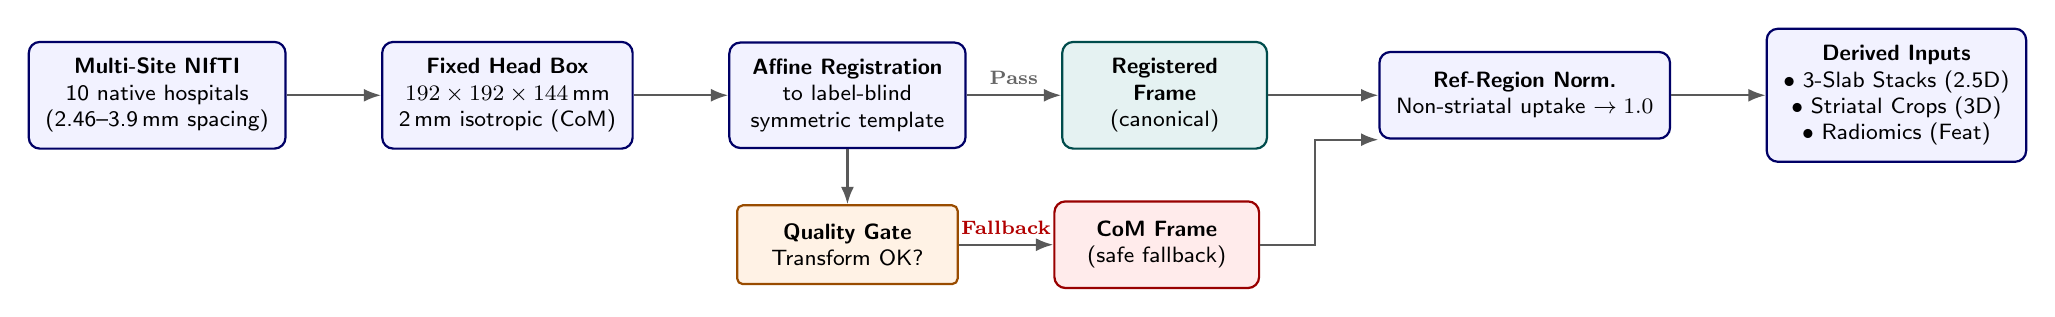
\begin{tikzpicture}[
  font=\footnotesize\sffamily,
  node distance=8mm and 12mm,
  stage/.style={draw=blue!40!black, rounded corners=4pt, fill=blue!5, line width=0.8pt, align=center, minimum height=1.1cm, inner sep=6pt},
  decision/.style={draw=orange!60!black, fill=orange!10, rounded corners=2pt, line width=0.8pt, align=center, minimum height=1.0cm, inner sep=5pt},
  passnode/.style={draw=teal!60!black, fill=teal!10, rounded corners=4pt, line width=0.8pt, align=center, minimum height=1.1cm, inner sep=6pt},
  failnode/.style={draw=red!60!black, fill=red!8, rounded corners=4pt, line width=0.8pt, align=center, minimum height=1.1cm, inner sep=6pt},
  arrow/.style={-{Latex[length=2.2mm]}, thick, gray!70!black},
  lbl/.style={font=\scriptsize\bfseries, text=gray!80!black}
]
  % Stage 1: Harmonization
  \node[stage, minimum width=2.8cm] (raw) {\textbf{Multi-Site NIfTI}\\10 native hospitals\\(2.46--3.9\,mm spacing)};
  \node[stage, right=of raw, minimum width=3.0cm] (headbox) {\textbf{Fixed Head Box}\\$192\times192\times144$\,mm\\2\,mm isotropic (CoM)};
  
  % Stage 2: Registration & Fallback
  \node[stage, right=of headbox, minimum width=3.0cm] (reg) {\textbf{Affine Registration}\\to label-blind\\symmetric template};
  \node[decision, below=7mm of reg, minimum width=2.8cm] (gate) {\textbf{Quality Gate}\\Transform OK?};
  
  % Paths
  \node[passnode, right=of reg, minimum width=2.6cm] (regframe) {\textbf{Registered}\\\textbf{Frame}\\(canonical)};
  \node[failnode, right=of gate, minimum width=2.6cm] (comframe) {\textbf{CoM Frame}\\(safe fallback)};
  
  % Stage 3: Normalization & Derivation
  \node[stage, right=14mm of regframe, minimum width=3.0cm] (norm) {\textbf{Ref-Region Norm.}\\Non-striatal uptake $\to 1.0$};
  \node[stage, right=of norm, minimum width=3.2cm] (inputs) {\textbf{Derived Inputs}\\$\bullet$ 3-Slab Stacks (2.5D)\\$\bullet$ Striatal Crops (3D)\\$\bullet$ Radiomics (Feat)};

  % Connecting arrows
  \draw[arrow] (raw) -- (headbox);
  \draw[arrow] (headbox) -- (reg);
  \draw[arrow] (reg) -- (gate);
  
  \draw[arrow] (reg) -- node[above, lbl] {Pass} (regframe);
  \draw[arrow] (gate) -- node[above, lbl, text=red!70!black] {Fallback} (comframe);
  
  \draw[arrow] (regframe) -- (norm);
  \draw[arrow] (comframe.east) -| ++(0.7,0) |- (norm.south west);
  \draw[arrow] (norm) -- (inputs);

\end{tikzpicture}}
\caption{Preprocessing pipeline. Every scan is first placed in a fixed head box, then registered to a label-blind study template; a per-scan fallback check reverts implausible registrations to the unregistered center-of-mass (CoM) frame rather than propagating a bad alignment. Reference-region normalization and slab generation follow identically in either frame.}
\label{fig:preprocessing}
\end{figure}

\subsection{Multi-arm ensemble}
\label{sec:ensemble}

An \emph{arm} is an independent model family that produces one probability per scan from the head box; \emph{checkpoints} (identified by fold and seed, or \emph{full-data} for a checkpoint trained on every labelled scan) within an arm are averaged. The reported ensemble's five pillars are (\Cref{fig:ensemble}):

\begin{itemize}[leftmargin=*]
\item \textbf{Hemisphere arm}: a bilateral, weight-shared 3D encoder over left/right striatal half-crops with an explicit asymmetry head, detailed in \Cref{sec:hemi}. This is the single strongest standalone arm (\Cref{sec:results}) and receives the largest combiner weight.
\item \textbf{Self-supervised 3D arm}: a full-volume 3D convolutional network initialized from self-supervised (VICReg-style) pretraining on the registered head box, rather than from-scratch or ImageNet-style initialization.
\item \textbf{Feature arm}: a kernel-based classifier (random Fourier features) over a bank of handcrafted radiomics descriptors extracted from the registered frame, rather than a learned convolutional encoder --- the ensemble's one non-deep-learning member.
\item \textbf{Coronal 2.5D arm}: a ConvNeXt-style network over coronal slab stacks.
\item \textbf{Axial 2.5D arm}: an EfficientNetV2-style network over axial slab stacks.
\end{itemize}

A sixth candidate, a \emph{tri-planar} 2.5D arm combining multiple anatomical views, was trained and evaluated but is not part of the five-pillar ensemble reported here; \Cref{sec:results} reports why, and what that decision reveals about validating ensemble weights under site shift.

\subsection{The hemisphere arm: a shared-weight bilateral encoder}
\label{sec:hemi}

The hemisphere arm is the ensemble's strongest single member and its only architecture designed from scratch for this pipeline rather than adapted from a general-purpose backbone, so we detail it precisely (\Cref{fig:hemi}). The registered striatal crop ($24\times48\times32$ voxels per hemisphere after splitting a $48\times48\times32$ crop at the midline) is divided into a left half and a right half; the right half is flipped along the split axis so both halves share one orientation. Both halves are then embedded by \emph{one} encoder instance in a single batched forward pass --- literally the same weights, not two separately-trained copies --- consisting of a convolutional stem (Conv3D, GroupNorm, SiLU) followed by four residual 3D blocks at widths $24{\to}48{\to}96{\to}192$ (the first block at stride 1, the remaining three at stride 2, each with a projection skip connection when width or stride changes) and a global average pool, yielding one 192-dimensional feature vector per hemisphere, $f_L$ and $f_R$.

Two heads then read out these features. A \emph{pair head} takes the symmetric combination $[f_L+f_R,\,|f_L-f_R|]$ (384-d: a bilateral-strength term and an explicit asymmetry-magnitude term) through a two-layer MLP (384$\to$128$\to$1) to a logit $z_{\text{pair}}$. A \emph{side head} --- again one shared instance, applied separately to $f_L$ and $f_R$ --- maps each 192-d feature through a smaller MLP (192$\to$64$\to$1) to a per-side logit, and the arm takes $z_{\text{side}} = \max(z_L, z_R)$: whichever hemisphere looks worse drives this term, matching the clinically typical asymmetric-onset presentation this challenge's ambiguous cases often show (\Cref{sec:intro}). The arm's output is $z = z_{\text{pair}} + z_{\text{side}}$. Because $[f_L+f_R,\,|f_L-f_R|]$ and $\max(z_L,z_R)$ are both symmetric under swapping $L$ and $R$, mirroring an entire input scan --- the label-preserving flip already used for training augmentation and test-time variants (\Cref{sec:validation}) --- leaves $z$ exactly unchanged: the architecture is invariant to the flip by construction, not by learning it from data.

\begin{figure}[t]
\centering
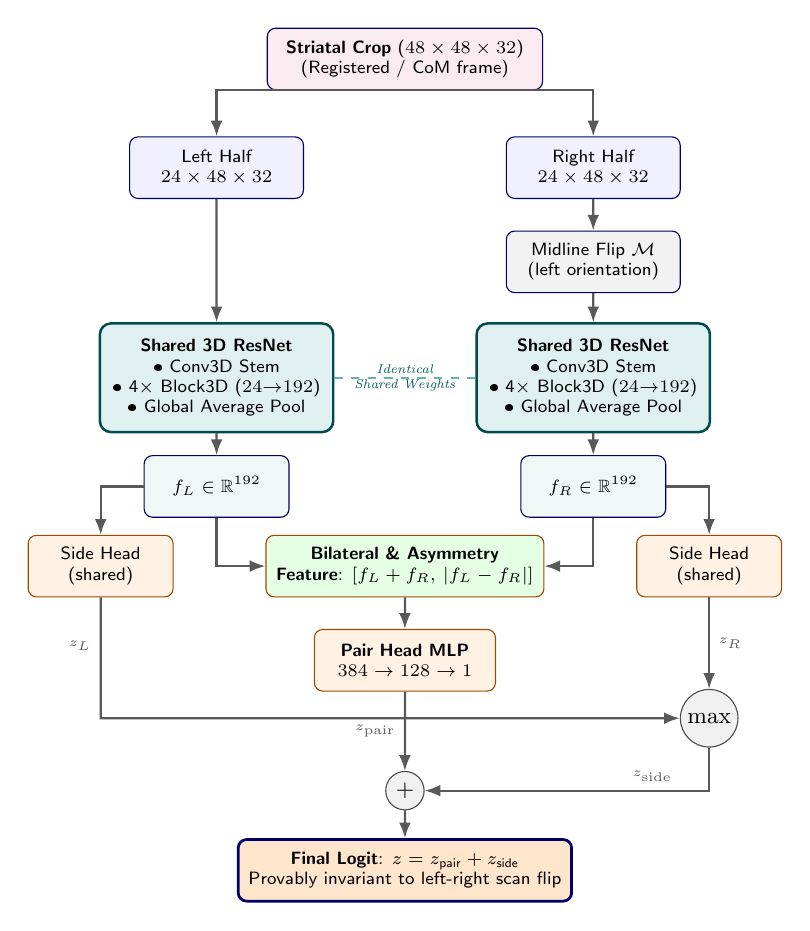
\begin{tikzpicture}[
  font=\scriptsize\sffamily,
  scale=0.92, every node/.style={transform shape},
  box/.style={draw=blue!40!black, rounded corners=3pt, fill=blue!6, align=center, inner sep=4pt, minimum height=0.85cm},
  enc/.style={draw=teal!60!black, rounded corners=4pt, fill=teal!12, align=center, line width=0.9pt, inner sep=5pt, minimum height=1.5cm},
  head/.style={draw=orange!60!black, rounded corners=3pt, fill=orange!10, align=center, inner sep=4pt, minimum height=0.85cm},
  op/.style={draw=gray!60!black, circle, fill=gray!12, inner sep=2pt, font=\small\bfseries},
  arrow/.style={-{Latex[length=2mm]}, thick, gray!70!black}
]
  % Top row: Input & Half Crops
  \node[box, fill=purple!8, minimum width=3.8cm] (input) at (0, 3.8) {\textbf{Striatal Crop} ($48\times48\times32$)\\(Registered / CoM frame)};
  \node[box, minimum width=2.4cm] (left1) at (-2.6, 2.3) {Left Half\\$24\times48\times32$};
  \node[box, minimum width=2.4cm] (right1) at (2.6, 2.3) {Right Half\\$24\times48\times32$};
  \node[box, fill=gray!10, minimum width=2.4cm] (mirror) at (2.6, 1.0) {Midline Flip $\mathcal{M}$\\(left orientation)};

  % Mid row: Shared 3D Encoder
  \node[enc, minimum width=3.2cm] (encL) at (-2.6, -0.6) {\textbf{Shared 3D ResNet}\\\textbullet\ Conv3D Stem\\\textbullet\ 4$\times$ Block3D ($24{\to}192$)\\\textbullet\ Global Average Pool};
  \node[enc, minimum width=3.2cm] (encR) at (2.6, -0.6) {\textbf{Shared 3D ResNet}\\\textbullet\ Conv3D Stem\\\textbullet\ 4$\times$ Block3D ($24{\to}192$)\\\textbullet\ Global Average Pool};
  \node[font=\tiny\itshape, text=teal!70!black, align=center] at (0, -0.6) {Identical\\Shared Weights};
  \draw[dashed, teal!60, thick] (encL.east) -- (encR.west);

  % Feature vectors
  \node[box, fill=teal!6, minimum width=2.0cm] (fL) at (-2.6, -2.1) {$f_L \in \mathbb{R}^{192}$};
  \node[box, fill=teal!6, minimum width=2.0cm] (fR) at (2.6, -2.1) {$f_R \in \mathbb{R}^{192}$};

  % Bottom row: Dual Symmetric Heads
  \node[head, fill=green!10, minimum width=3.2cm] (combine) at (0, -3.2) {\textbf{Bilateral \& Asymmetry}\\\textbf{Feature}: $[f_L+f_R,\, |f_L-f_R|]$};
  \node[head, minimum width=2.5cm] (pairhead) at (0, -4.5) {\textbf{Pair Head MLP}\\$384 \to 128 \to 1$};
  
  \node[head, minimum width=2.0cm] (sideL) at (-4.2, -3.2) {Side Head\\(shared)};
  \node[head, minimum width=2.0cm] (sideR) at (4.2, -3.2) {Side Head\\(shared)};
  \node[op] (maxop) at (4.2, -5.3) {$\max$};

  \node[op] (sumop) at (0, -6.3) {$+$};
  \node[box, fill=orange!20, minimum width=4.0cm, line width=1pt] (output) at (0, -7.4) {\textbf{Final Logit}: $z = z_{\text{pair}} + z_{\text{side}}$\\{\scriptsize Provably invariant to left-right scan flip}};

  % Arrows
  \draw[arrow] (input.south) -| (left1.north);
  \draw[arrow] (input.south) -| (right1.north);
  \draw[arrow] (left1) -- (encL);
  \draw[arrow] (right1) -- (mirror);
  \draw[arrow] (mirror) -- (encR);
  \draw[arrow] (encL) -- (fL);
  \draw[arrow] (encR) -- (fR);
  
  \draw[arrow] (fL.south) |- (combine.west);
  \draw[arrow] (fR.south) |- (combine.east);
  \draw[arrow] (combine) -- (pairhead);
  
  \draw[arrow] (fL.west) -| (sideL.north);
  \draw[arrow] (fR.east) -| (sideR.north);
  \draw[arrow] (sideL.south) -- (-4.2, -5.3) node[pos=0.4,left,font=\tiny]{$z_L$} -- (maxop.west);
  \draw[arrow] (sideR.south) -- node[right,font=\tiny]{$z_R$} (maxop.north);

  \draw[arrow] (pairhead) -- node[left,font=\tiny]{$z_{\text{pair}}$} (sumop);
  \draw[arrow] (maxop.south) |- node[pos=0.6,above,font=\tiny]{$z_{\text{side}}$} (sumop.east);
  \draw[arrow] (sumop) -- (output);
\end{tikzpicture}
\caption{The hemisphere arm: a single shared-weight 3D encoder embeds the left and mirrored-right striatal half-crops in one forward pass. A pair head reads a symmetric bilateral-strength-plus-asymmetry feature; a side head (also weight-shared across sides) scores each hemisphere independently, and the arm takes the worse-side score via a max. Because every combining operation is symmetric in $L$/$R$, the whole arm is exactly invariant to mirroring the input scan.}
\label{fig:hemi}
\end{figure}

\begin{figure}[t]
\centering
\resizebox{\textwidth}{!}{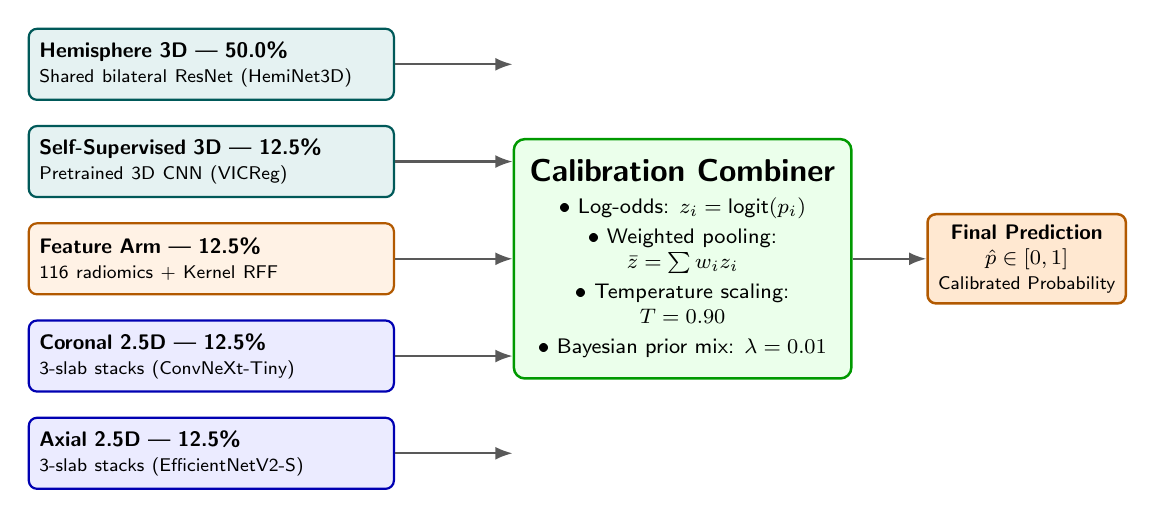
\begin{tikzpicture}[
  font=\footnotesize\sffamily,
  scale=0.95, every node/.style={transform shape},
  arm3d/.style={draw=teal!70!black, rounded corners=3pt, text width=4.6cm, minimum height=0.95cm, align=left, fill=teal!10, line width=0.8pt, inner sep=4pt},
  arm25d/.style={draw=blue!70!black, rounded corners=3pt, text width=4.6cm, minimum height=0.95cm, align=left, fill=blue!8, line width=0.8pt, inner sep=4pt},
  armfeat/.style={draw=orange!70!black, rounded corners=3pt, text width=4.6cm, minimum height=0.95cm, align=left, fill=orange!10, line width=0.8pt, inner sep=4pt},
  comb/.style={draw=green!60!black, rounded corners=4pt, minimum width=4.3cm, minimum height=3.2cm, align=center, fill=green!8, line width=0.9pt, inner sep=6pt},
  outbox/.style={draw=orange!70!black, rounded corners=3pt, minimum width=2.6cm, minimum height=1.1cm, align=center, fill=orange!18, line width=0.9pt, inner sep=4pt},
  arrow/.style={-{Latex[length=2.2mm]}, thick, gray!70!black}
]
  % 5 Arms with clean text and no touching
  \node[arm3d] (a1) at (0, 2.6) {\textbf{Hemisphere 3D} --- \textbf{50.0\%}\\{\scriptsize Shared bilateral ResNet (HemiNet3D)}};
  \node[arm3d] (a2) at (0, 1.3) {\textbf{Self-Supervised 3D} --- \textbf{12.5\%}\\{\scriptsize Pretrained 3D CNN (VICReg)}};
  \node[armfeat] (a3) at (0, 0.0) {\textbf{Feature Arm} --- \textbf{12.5\%}\\{\scriptsize 116 radiomics + Kernel RFF}};
  \node[arm25d] (a4) at (0, -1.3) {\textbf{Coronal 2.5D} --- \textbf{12.5\%}\\{\scriptsize 3-slab stacks (ConvNeXt-Tiny)}};
  \node[arm25d] (a5) at (0, -2.6) {\textbf{Axial 2.5D} --- \textbf{12.5\%}\\{\scriptsize 3-slab stacks (EfficientNetV2-S)}};

  % Combiner Box
  \node[comb] (comb) at (6.3, 0.0) {
    \textbf{\large Calibration Combiner}\\[5pt]
    \parbox{3.9cm}{\centering
      \textbullet\ Log-odds: $z_i = \text{logit}(p_i)$\\[2pt]
      \textbullet\ Weighted pooling: $\bar{z} = \sum w_i z_i$\\[2pt]
      \textbullet\ Temperature scaling: $T=0.90$\\[2pt]
      \textbullet\ Bayesian prior mix: $\lambda=0.01$
    }
  };

  % Output Box
  \node[outbox] (out) at (10.9, 0.0) {\textbf{Final Prediction}\\$\hat{p} \in [0, 1]$\\{\scriptsize Calibrated Probability}};

  % Connections
  \foreach \a in {a1, a2, a3, a4, a5} {
    \draw[arrow] (\a.east) -- (comb.west |- \a.east);
  }
  \draw[arrow] (comb) -- (out);
\end{tikzpicture}}
\caption{The multi-arm ensemble: five arm families, color-coded by type (3D encoders in teal, 2.5D encoders in blue, the one non-deep-learning arm in amber), each produce a per-scan probability from a shared registered-frame input. Weights are the OOF-fitted Master Final stack's combiner weights (\Cref{tab:arms}). The combiner merges arm outputs by weighted log-odds averaging, a fitted temperature, and a small training-prevalence prior mix.}
\label{fig:ensemble}
\end{figure}

\subsection{Training protocol and validation}
\label{sec:validation}

All arms are trained under an \emph{honest protocol}: a fixed epoch budget with the final averaged weights shipped, so that out-of-fold (OOF) predictions never reflect a choice (early stopping, checkpoint selection) made using the held-out fold itself. Two fold partitions are used. Five canonical random stratified folds are used for the model-selection and combiner-fitting numbers reported throughout this paper. A separate \emph{site-fold} partition holds out whole pseudo-sites (\Cref{sec:data}) and is used exclusively to estimate cross-site generalization (\Cref{sec:shiftgap}); it is never used to select a final model or checkpoint, to avoid contaminating the very estimate it is meant to provide. At inference, a fixed set of \emph{test-time variants} --- slab-center shifts and a left/right mirror --- is averaged per scan, defined once and applied identically to OOF prediction and to real inference.

\subsection{Combiner}
\label{sec:combiner}

Arm probabilities are combined as a weighted average of log-odds, followed by a single temperature and a small prior-mix step. The temperature is fitted on site-fold predictions where available and is conventionally floored at 1 (never sharpening a distribution, only flattening it) under random-fold validation; we revisit this floor explicitly in \Cref{sec:results} because it does not transfer cleanly under site shift. The prior mix blends in a small fraction of the training-set prevalence as insurance against confident, wrong probabilities --- a device specifically motivated by log loss's asymmetric penalty for overconfidence, which accuracy or AUROC would not motivate.

\subsection{The shift-gap diagnostic}
\label{sec:shiftgap}

Let \lrand{} denote the out-of-fold log loss under the random stratified folds of \Cref{sec:validation}, and \lsite{} denote the out-of-fold log loss under the site folds, which never mix a pseudo-site's scans between training and validation within a fold. We define the \textbf{shift gap} as
\begin{equation}
\shiftgap \;=\; \lsite \;-\; \lrand.
\label{eq:shiftgap}
\end{equation}
\shiftgap{} approximates, prospectively and without any access to the hidden test set, the excess loss a model is likely to incur when the true test distribution over- or under-represents acquisition sites relative to their training-set frequency. It requires only acquisition metadata (here, the pseudo-site fingerprint), never true hospital identity or patient-level information, and is therefore computable in any multi-site medical imaging challenge that permits an unsupervised acquisition-fingerprint partition --- independent of whether the true hidden-test site mix is ever disclosed.

We report \shiftgap{} in \Cref{sec:results} alongside the actually observed gap between local validation and the platform's real leaderboard, and we treat the comparison between the two as itself a finding rather than a validation that the diagnostic fully explains leaderboard behavior (\Cref{sec:discussion}).

\section{Experiments and Results}
\label{sec:results}

\textbf{A note on timing.} The results below are interim. The competition closes September 16, 2026, and the private leaderboard used for final prize ranking has not yet been scored at the time of writing (September 11, 2026). All numbers below are drawn from the public leaderboard, DrivenData's free smoke-test facility (a scored run of a submission zip against 20 held-out training scans, capped at three per day and never counted toward the rolling three-per-week real-submission quota), and our own local out-of-fold validation. A revision will report the final private-leaderboard rank once available.

\subsection{Smoke-to-public calibration ladder}

\Cref{tab:ladder} reports every real submission and platform smoke test made to date, tracking each candidate's local out-of-fold estimate, its DrivenData smoke-test score (20 scans), and, where submitted for real scoring, its public leaderboard score.

\begin{table}[t]
\centering
\small
\caption{Smoke-to-public calibration ladder. Smoke scores are read from the platform's 20-scan smoke test and never fitted on. Rank is the most recently verified value at time of writing (Sept 10--11, 2026); it drifts as other competitors submit and is distinct from the fixed public log loss/AUROC. Master v2 --- the five-pillar ensemble whose site-fold vs.\ random-fold shift gap is reported in \Cref{sec:shiftgap-results} --- had not yet been submitted for real (leaderboard-scored) evaluation at the time of writing; it is a different, later configuration than Run 3 or Run 4a.}
\label{tab:ladder}
\begin{tabular}{@{}lccc@{}}
\toprule
\textbf{Candidate} & \textbf{Smoke (20 scans)} & \textbf{Public leaderboard} & \textbf{Rank (of 450)} \\
\midrule
Run 3 (44-checkpoint stack) & 0.2397 & 0.2817 & 66 \\
Run 4a (30-checkpoint stack) & 0.2176 / 0.2263 & \textbf{0.2473} (AUROC 0.9536) & \textbf{44} \\
Run 7 (hemisphere, standalone) & 0.2706 & --- & --- \\
Run 6b (tri-planar, standalone) & 0.2341 & --- & --- \\
Master Final (5-pillar stack) & 0.2363 & --- (not submitted) & --- \\
Master v2 (5-pillar, equal weights) & 0.2381 & --- (not yet submitted) & --- \\
\bottomrule
\end{tabular}
\end{table}

Run 4a is the best-performing submission scored for real at the time of writing: public log loss 0.2473, AUROC 0.9536, rank 44 of 450. For reference, the interim public leaderboard's top entries stood at 0.2166 (rank 1), 0.2379 (rank 10), and 0.2457 (rank 15).

\subsection{Site-fold vs.\ random-fold: the shift gap quantified}
\label{sec:shiftgap-results}

\Cref{sec:shiftgap} defines the shift gap on the five-pillar ensemble of \Cref{sec:ensemble} (hemisphere, self-supervised 3D, feature, coronal 2.5D, and axial 2.5D arms) --- the Master v2 candidate of \Cref{tab:ladder}, not yet submitted for real scoring. Out-of-fold log loss under random stratified folds is 0.2266 with equal arm weights (0.2323 with OOF-fitted weights); the same ensemble under leave-pseudo-site-out folds scores 0.2402 with equal weights, giving a shift gap $\shiftgap \approx 0.005$--$0.008$ (\Cref{fig:shiftgap}).

\begin{figure}[t]
\centering
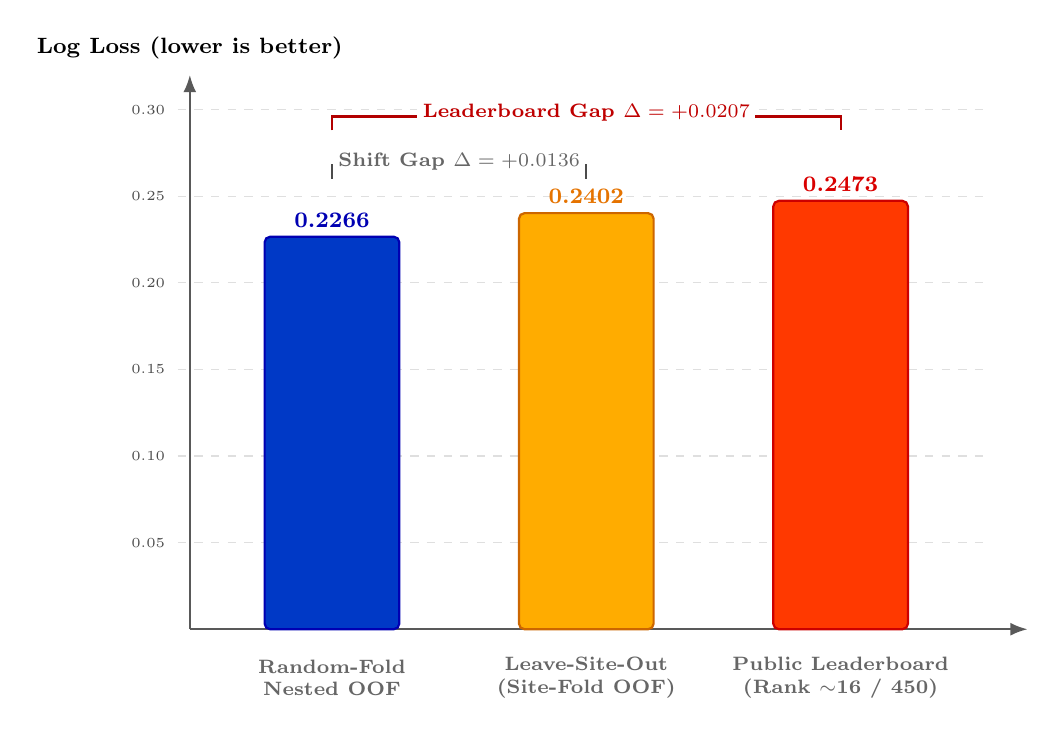
\begin{tikzpicture}[
  font=\sffamily,
  scale=1.0,
  y=22cm, x=1.9cm,
  barlabel/.style={font=\footnotesize\bfseries},
  axislabel/.style={font=\scriptsize\bfseries, text=gray!80!black}
]
  % Y Axis and gridlines
  \draw[-{Latex[length=2.2mm]}, thick, gray!70!black] (0,0) -- (0,0.32) node[above=2pt, font=\footnotesize\bfseries, text=black] {Log Loss (lower is better)};
  \draw[-{Latex[length=2.2mm]}, thick, gray!70!black] (0,0) -- (5.6,0);

  \foreach \val in {0.05, 0.10, 0.15, 0.20, 0.25, 0.30} {
    \draw[gray!25, dashed] (-0.08, \val) -- (5.3, \val);
    \node[anchor=east, font=\tiny, text=gray!60!black] at (-0.10, \val) {\val};
  }

  % Bar 1: Random-Fold OOF (0.2266)
  \draw[fill=blue!55!teal, draw=blue!70!black, rounded corners=2pt, line width=0.8pt] (0.5, 0) rectangle (1.4, 0.2266);
  \node[barlabel, text=blue!70!black] at (0.95, 0.236) {0.2266};
  \node[axislabel, align=center] at (0.95, -0.028) {Random-Fold\\Nested OOF};

  % Bar 2: Leave-Site-Out OOF (0.2402)
  \draw[fill=orange!65!yellow, draw=orange!80!black, rounded corners=2pt, line width=0.8pt] (2.2, 0) rectangle (3.1, 0.2402);
  \node[barlabel, text=orange!90!black] at (2.65, 0.250) {0.2402};
  \node[axislabel, align=center] at (2.65, -0.028) {Leave-Site-Out\\(Site-Fold OOF)};

  % Bar 3: Public Leaderboard (0.2473)
  \draw[fill=red!55!orange, draw=red!80!black, rounded corners=2pt, line width=0.8pt] (3.9, 0) rectangle (4.8, 0.2473);
  \node[barlabel, text=red!85!black] at (4.35, 0.257) {\textbf{0.2473}};
  \node[axislabel, align=center] at (4.35, -0.028) {Public Leaderboard\\(\textbf{Rank} $\sim$16 / 450)};

  % Shift Gap Annotation Bracket (Between Bar 1 and Bar 2)
  \draw[thick, gray!60!black] (0.95, 0.260) -- (0.95, 0.268) -- (2.65, 0.268) -- (2.65, 0.260);
  \node[font=\scriptsize\bfseries, fill=white, inner sep=2pt, text=gray!80!black] at (1.80, 0.270) {Shift Gap $\Delta = +0.0136$};

  % Public Gap Annotation Bracket (Between Bar 1 and Bar 3)
  \draw[thick, red!70!black] (0.95, 0.288) -- (0.95, 0.296) -- (4.35, 0.296) -- (4.35, 0.288);
  \node[font=\scriptsize\bfseries, fill=white, inner sep=2pt, text=red!75!black] at (2.65, 0.298) {Leaderboard Gap $\Delta = +0.0207$};

\end{tikzpicture}
\caption{Random-fold out-of-fold log loss (0.2266) vs.\ leave-pseudo-site-out log loss (0.2402) for the current best five-arm ensemble, alongside the actual public leaderboard score of the best real submission (0.2473, a different, earlier configuration). The shift gap ($\approx$0.005--0.008) between the first two bars is small relative to the much larger gap to the third, indicating the pseudo-site partition does not capture the full extent of the true hidden test-set shift.}
\label{fig:shiftgap}
\end{figure}

\begin{table}[t]
\centering
\small
\caption{Standalone out-of-fold performance of each arm considered for the five-pillar ensemble, plus the excluded tri-planar candidate. Weight is each arm's share of the separate, OOF-\emph{fitted} Master Final stack --- a different weighting from the equal-weight Master v2 ensemble whose shift gap is reported above (\Cref{sec:shiftgap-results}) --- in which the tri-planar candidate was evaluated and assigned zero weight. Site-fold numbers are reported only for the feature arm, the one arm individually site-validated before assembly.}
\label{tab:arms}
\begin{tabular}{@{}lccc@{}}
\toprule
\textbf{Arm} & \textbf{Random-fold OOF (loss / AUROC)} & \textbf{Site-fold OOF (loss / AUROC)} & \textbf{Master Final weight} \\
\midrule
Hemisphere & 0.2379 / 0.9658 & --- & 50.0\% \\
Self-supervised 3D & 0.2519 / 0.9608 & --- & 12.5\% \\
Feature (radiomics) & 0.2997 / 0.9455 & 0.3106 / 0.9410 & 12.5\% \\
Coronal 2.5D & 0.2651 / 0.9571 & --- & 12.5\% \\
Axial 2.5D & 0.2630 / 0.9576 & --- & 12.5\% \\
\midrule
Tri-planar (excluded) & 0.2560 / 0.9603 & --- & 0.0\% \\
\bottomrule
\end{tabular}
\end{table}

Two further observations sharpen this picture, using the standalone arm performance of \Cref{tab:arms}. First, the temperature fitted on site-fold predictions is below 1 ($T_{\text{site}} \approx 0.826$) whereas random-fold fitting stays near 1; forcing the conventional $T \geq 1$ floor onto the site-pool predictions \emph{worsens} site-fold log loss, from 0.2402 to 0.2449 --- meaning the ``never sharpen below $T=1$'' heuristic, sound under random-fold validation, does not transfer once site shift is present. Second, the tri-planar arm was assigned zero ensemble weight by the OOF-fitted stacker (its predictions were collinear with the hemisphere arm's under random folds) despite scoring the best random-fold log loss of any 2.5D arm in \Cref{tab:arms} (0.2560, ahead of both the coronal and axial 2.5D arms it was excluded in favor of blending with) and being the single strongest \emph{individual} arm on the real hidden smoke test (0.2341, \Cref{tab:ladder}); an OOF-fitted stacker that never sees site shift has no way to detect that this arm's true cross-site value differs from what its random-fold collinearity suggests. Third, the feature arm is the only individually site-validated arm and shows the pattern \Cref{sec:shiftgap-results} describes at ensemble level even more starkly: its own site-fold loss (0.3106) is 0.011 worse than its random-fold loss (0.2997), a per-arm shift gap larger than the ensemble's, despite the feature arm being the ensemble's one non-deep-learning, most classically ``interpretable'' member.

\subsection{Interpreting the residual gap}

The shift gap computed from pseudo-site folds (0.005--0.008) is smaller than the gap actually observed between each submitted model's own local nested out-of-fold estimate and its real public leaderboard score: 0.2603 (nested) vs.\ 0.2817 (public) for run 3, a gap of 0.021, and 0.2491 (nested) vs.\ 0.2473 (public) for run 4a, a gap of 0.018 (these are local nested combiner estimates, distinct from the 20-scan platform smoke-test scores also shown in \Cref{tab:ladder}, which are noisier still: the identical run-4a submission zip scored 0.2176 and 0.2263 on two separate 20-scan smoke draws, a 0.0087 spread attributable to sample size alone). The training-site shift gap is therefore two to four times smaller than the nested-to-public gap actually observed on this pipeline's two real submissions to date. We report this discrepancy directly rather than treating the shift-gap diagnostic as sufficient, and note two caveats on the comparison itself. First, run 3 and run 4a are earlier, differently-composed stacks, not the five-pillar ensemble the shift gap above is computed on (\Cref{sec:shiftgap-results}); the comparison uses them as the best available evidence for this pipeline's typical nested-to-public behavior, not as a before/after measurement on one model. Second, the residual gap indicates either that the true hidden-test site composition is more adversarial than the training-set's own site distribution suggests, that the pseudo-site fingerprint under-resolves some real acquisition variability the true (undisclosed) hospital identity would capture, or both.

\section{Discussion}
\label{sec:discussion}

The central empirical finding of this paper is not that the shift gap explains the leaderboard gap --- it does not, at least not fully --- but that a small, honestly-reported, acquisition-metadata-only diagnostic can still surface concrete, actionable failures that an OOF-only validation protocol would hide: an ensemble-weighting heuristic ($T \geq 1$) that reverses under site shift, and a stacking decision (zero weight on the tri-planar arm) that discards the single arm best supported by real hidden-test evidence. Both findings would have been invisible to a pipeline that validated only on random folds, which is the validation protocol nearly every paper reviewed in \Cref{sec:related} uses.

This also reframes what ``generalization'' means for this specific literature. \citet{choi2017}'s independent-cohort validation --- the strongest cross-site result in the prior literature --- succeeded on a single additional hospital under a controlled, MNI-normalized pipeline. The present challenge asks the same question across ten hospitals simultaneously, in native acquisition space, with the true test-site mix withheld; a shift gap of 0.005--0.008 on the training-site partition, against a leaderboard gap several times larger, suggests that success in the former setting does not straightforwardly predict success in the latter, and that pseudo-site-based estimation, while better than no site-aware validation at all, is not a substitute for true, disclosed site identity when one is available to a challenge organizer.

For challenge design more broadly, this suggests a concrete, low-cost improvement: organizers of multi-site medical imaging challenges could release (or allow competitors to derive) an acquisition-fingerprint-based site partition specifically so a shift-gap-style diagnostic is computable without disclosing hospital identity or patient information --- exactly the affordance the pseudo-site construct provided here.

\section{Limitations}
\label{sec:limitations}

\begin{itemize}[leftmargin=*]
\item \textbf{Interim results.} All numbers reported here predate the competition's September 16, 2026 close; the private leaderboard used for final prize ranking has not yet been scored. A revision will update \Cref{tab:ladder} and \Cref{sec:results} with final figures.
\item \textbf{Pseudo-site is a proxy, not ground truth.} True hospital identity is withheld for every scan; pseudo-site approximates it from acquisition metadata (voxel spacing, grid shape, intensity regime) and may merge or split true sites incorrectly.
\item \textbf{Single-country, ten-hospital scope.} All contributing sites are French; generalization claims beyond this specific hospital-and-scanner population are not established by this study.
\item \textbf{Undisclosed, likely small training set.} The organizer does not publish the exact training-set size; a forum participant's independent characterization (``very small for training neural nets'') is consistent with the modest per-arm capacity and calibration-first design used here, but limits the statistical power of any single ablation reported.
\item \textbf{No hidden-test visibility.} The shift gap is, by construction, a proxy computed from training-time metadata; it cannot and does not guarantee agreement with the true, undisclosed hidden test-set site composition, as \Cref{sec:shiftgap-results} demonstrates directly.
\item \textbf{No point estimate here carries a confidence interval.} All log losses reported (nested, site-fold, smoke, public) are point estimates; the measured 0.0087 smoke-test spread on an identical zip (\Cref{sec:shiftgap-results}) indicates the smoke-test numbers in particular carry non-trivial sampling noise at $n=20$ that this paper does not formally quantify for every comparison.
\item \textbf{The shift gap and the nested-to-public comparison use different model configurations.} The shift gap (\Cref{sec:shiftgap-results}) is computed on the five-pillar ensemble, which has not been submitted for real scoring; the 0.018--0.021 nested-to-public gap it is compared against comes from two earlier, differently-composed submitted stacks (run 3, run 4a). The comparison is offered as the best available evidence of this pipeline's typical behavior, not a controlled before/after measurement on one model.
\end{itemize}

\section{Ethics and Data Availability Statement}
\label{sec:ethics}

The dataset used in this study is a restricted-access clinical dataset provided by the French Society of Nuclear Medicine, Health Data Hub, and GaelO as part of DrivenData Competition \#311 (``DaT Parkinson's Challenge''), supported by France's France~2030 plan. Per the competition's official rules, the raw imaging data may not be redistributed, copied, or shared with parties outside the competition and is therefore not released alongside this paper. The dataset is intended for future public release via France's data.gouv.fr portal and the BOAS open health algorithm library, at which point external replication will become possible. All code, trained model weights, and configuration needed to reproduce the described pipeline --- excluding the underlying imaging data --- will be released under the MIT License at a public repository following the competition's close, consistent with the competition's code-sharing permission and its MIT License requirement for prize-winning solutions. The original imaging data collection and its governance as human-subject clinical data were the responsibility of the organizing institutions (French Society of Nuclear Medicine, Health Data Hub, GaelO) under France's Health Data Challenges program; the author of this paper did not collect the data and had no role in its original ethical review, and reports here only a secondary analysis of de-identified scans made available through the competition platform.

\section{Author Contributions}
Harshdip Saha: Conceptualization, Methodology, Software, Validation, Formal analysis, Investigation, Writing -- original draft, Writing -- review \& editing, Visualization. (CRediT taxonomy.)

\section{Conflict of Interest}
The author declares no conflict of interest. The author is a participant in DrivenData Competition \#311 and may be eligible for competition prizes; no other financial or non-financial competing interests exist.

\section{Funding}
This work received no external funding. Model development used free-tier cloud GPU resources; final scored inference runs on the competition's own execution infrastructure, provided by DrivenData under competition rules and used solely for evaluating submissions.

\section{Use of AI Tools}
AI-assisted tools (Claude and Claude Code, Anthropic) were used throughout this project for pipeline engineering, experiment scripting, literature search assistance, and drafting and editing support for this manuscript. All experimental design decisions, result interpretation, and final claims are the responsibility of the human author, who reviewed and verified all reported numbers against the underlying experiment logs prior to submission.

\section{Conclusion}

We describe a five-pillar, site-aware ensemble for classifying DaT-SPECT scans from a new, ten-hospital, restricted-access dataset with no guaranteed pre-registration and no disclosed test-set site composition --- a harder and more realistic setting than the single-center, MNI-normalized cohorts the prior literature is built on. We introduce the shift gap, an acquisition-metadata-only diagnostic for cross-site generalization, and report it honestly alongside a larger real nested-to-public gap it only partly explains, surfacing two concrete pipeline failures (a calibration heuristic that reverses under site shift, and a stacking decision that discards the arm best supported by hidden-test evidence) that random-fold validation alone would have hidden. At the time of writing, this pipeline's best submission scored for real ranks ~16th of 450 on the interim public leaderboard (log loss 0.2473); a revision will report the final private-leaderboard result, including whether the unsubmitted five-pillar ensemble improves on it, once the competition closes on September 16, 2026.

\bigskip
\begin{thebibliography}{99}

\bibitem[Choi et~al.(2017)]{choi2017} H.~Choi, S.~Ha, H.~J.~Im, S.~H.~Paek, and D.~S.~Lee, ``Refining diagnosis of Parkinson's disease with deep learning-based interpretation of dopamine transporter imaging,'' \emph{NeuroImage: Clinical}, vol.~16, pp.~586--594, 2017.

\bibitem[Quan et~al.(2019)]{quan2019} T.~M.~Quan, N.~M.~Doan, M.~Le, T.~Nguyen, and V.~Q.~Ha, ``DaTscan SPECT image classification for Parkinson's disease,'' \emph{arXiv preprint arXiv:1909.04142}, 2019.

\bibitem[Nazari et~al.(2021)]{nazari2021} M.~Nazari, F.~Kluge, I.~Apostolova, S.~Klutmann, S.~Kimiaei, M.~Schroeder, and R.~Buchert, ``Explainable AI to improve acceptance of convolutional neural networks for automatic classification of dopamine transporter SPECT in the diagnosis of clinically uncertain parkinsonian syndromes,'' \emph{European Journal of Nuclear Medicine and Molecular Imaging}, vol.~49, pp.~1176--1186, 2021.

\bibitem[{Diagnostics}(2022)]{ensemblefusion2022} ``An ensemble of convolutional neural network models for the diagnosis of Parkinson's disease using DaTscan images,'' \emph{Diagnostics}, vol.~12, no.~5, art.~1173, 2022.

\bibitem[Zhao et~al.(2022)]{zhao2022} Y.~Zhao, J.~Wu, J.~Yuan, et~al., ``Decoding dopamine transporter imaging for differential diagnosis of parkinsonism using deep learning,'' \emph{European Journal of Nuclear Medicine and Molecular Imaging}, vol.~49, pp.~2798--2811, 2022.

\bibitem[{EJNMMI}(2022)]{radiomics2022} ``A radiomics signature for the diagnosis of Parkinson's disease from striatal DAT-SPECT with cross-manufacturer generalization,'' \emph{European Journal of Nuclear Medicine and Molecular Imaging}, vol.~49, 2022.

\bibitem[{Electronics}(2026)]{trainingprotocol2026} ``Revisiting CNN-based Parkinson's disease classification from DaT-SPECT images: the role of training protocols,'' \emph{Electronics}, vol.~15, no.~9, art.~1883, 2026.

\bibitem[Guo et~al.(2017)]{guo2017} C.~Guo, G.~Pleiss, Y.~Sun, and K.~Q.~Weinberger, ``On calibration of modern neural networks,'' in \emph{Proc. 34th International Conference on Machine Learning (ICML)}, 2017, pp.~1321--1330.

\bibitem[Lakshminarayanan et~al.(2017)]{lakshminarayanan2017} B.~Lakshminarayanan, A.~Pritzel, and C.~Blundell, ``Simple and scalable predictive uncertainty estimation using deep ensembles,'' in \emph{Advances in Neural Information Processing Systems (NeurIPS)}, vol.~30, 2017.

\bibitem[Gulrajani and Lopez-Paz(2021)]{gulrajani2021} I.~Gulrajani and D.~Lopez-Paz, ``In search of lost domain generalization,'' in \emph{International Conference on Learning Representations (ICLR)}, 2021.

\end{thebibliography}

\end{document}